\documentclass{beamer}
\mode<presentation>{
  \usetheme{Boadilla}
  \usefonttheme[onlylarge]{structurebold}
  \usefonttheme[stillsansseriflarge]{serif}
  \setbeamerfont*{frametitle}{size=\normalsize,series=\bfseries}
  % \setbeamertemplate{navigation symbols}{}
  \setbeamercovered{transparent}
}
\usepackage[english]{babel}
\usepackage[latin1]{inputenc}
\usepackage{times}
\usepackage[T1]{fontenc}
\usepackage{amsmath}
\usepackage{amssymb}
\usepackage{esint}
\usepackage{hyperref}
\usepackage{tikz}
\usepackage{xkeyval}
\usepackage{xargs}
\usepackage{xcolor}
\usepackage{verbatim}
\usepackage{listings}
\usepackage{multimedia}
\usepackage{bm}
\usepackage{siunitx}
\usetikzlibrary{
  arrows,
  calc,
  decorations.pathmorphing,
  decorations.pathreplacing,
  decorations.markings,
  fadings,
  positioning,
  shapes,
  arrows.meta
}
\usepgfmodule{oo}

\pgfdeclareradialshading{glow2}{\pgfpoint{0cm}{0cm}}{
  color(0mm)=(white);
  color(2mm)=(white);
  color(8mm)=(black);
  color(10mm)=(black)
}
\pgfdeclareradialshading{glow}{\pgfpoint{0cm}{0cm}}{
  color(0mm)=(white);
  color(5mm)=(white);
  color(9mm)=(black);
  color(10mm)=(black)
}

\begin{tikzfadingfrompicture}[name=glow fading]
  \shade [shading=glow] (0,0) circle (1);
\end{tikzfadingfrompicture}

\begin{tikzfadingfrompicture}[name=glow2 fading]
  \shade [shading=glow2] (0,0) circle (1);
\end{tikzfadingfrompicture}

\mode<handout>{
  \usepackage{pgfpages}
  \pgfpagesuselayout{4 on 1}[a4paper,landscape,border shrink=5mm]
  \setbeamercolor{background canvas}{bg=black!10}
}

\newcommand\pgfmathsinandcos[3]{%
  \pgfmathsetmacro#1{sin(#3)}%
  \pgfmathsetmacro#2{cos(#3)}%
}
\newcommand\LongitudePlane[3][current plane]{%
  \pgfmathsinandcos\sinEl\cosEl{#2} % elevation
  \pgfmathsinandcos\sint\cost{#3} % azimuth
  \tikzset{#1/.estyle={cm={\cost,\sint*\sinEl,0,\cosEl,(0,0)}}}
}
\newcommand\LatitudePlane[3][current plane]{%
  \pgfmathsinandcos\sinEl\cosEl{#2} % elevation
  \pgfmathsinandcos\sint\cost{#3} % latitude
  \pgfmathsetmacro\yshift{\cosEl*\sint}
  \tikzset{#1/.estyle={cm={\cost,0,0,\cost*\sinEl,(0,\yshift)}}} %
}
\newcommand\DrawLongitudeCircle[2][1]{
  \LongitudePlane{\angEl}{#2}
  \tikzset{current plane/.prefix style={scale=#1}}
  % angle of "visibility"
  \pgfmathsetmacro\angVis{atan(sin(#2)*cos(\angEl)/sin(\angEl))} %
  \draw[current plane] (\angVis:1) arc (\angVis:\angVis+180:1);
  \draw[current plane,dashed] (\angVis-180:1) arc (\angVis-180:\angVis:1);
}
\newcommand\DrawLatitudeCircleArrow[2][1]{
  \LatitudePlane{\angEl}{#2}
  \tikzset{current plane/.prefix style={scale=#1}}
  \pgfmathsetmacro\sinVis{sin(#2)/cos(#2)*sin(\angEl)/cos(\angEl)}
  % angle of "visibility"
  \pgfmathsetmacro\angVis{asin(min(1,max(\sinVis,-1)))}
  \draw[current plane,decoration={markings, mark=at position 0.6 with {\arrow{<}}},postaction={decorate},line width=.6mm] (\angVis:1) arc (\angVis:-\angVis-180:1);
  \draw[current plane,dashed,line width=.6mm] (180-\angVis:1) arc (180-\angVis:\angVis:1);
}
\newcommand\DrawLatitudeCircle[2][1]{
  \LatitudePlane{\angEl}{#2}
  \tikzset{current plane/.prefix style={scale=#1}}
  \pgfmathsetmacro\sinVis{sin(#2)/cos(#2)*sin(\angEl)/cos(\angEl)}
  % angle of "visibility"
  \pgfmathsetmacro\angVis{asin(min(1,max(\sinVis,-1)))}
  \draw[current plane] (\angVis:1) arc (\angVis:-\angVis-180:1);
  \draw[current plane,dashed] (180-\angVis:1) arc (180-\angVis:\angVis:1);
}
\newcommand\coil[1]{
  {\rh * cos(\t * pi r)}, {\apart * (2 * #1 + \t) + \rv * sin(\t * pi r)}
}
\makeatletter
\define@key{DrawFromCenter}{style}[{->}]{
  \tikzset{DrawFromCenterPlane/.style={#1}}
}
\define@key{DrawFromCenter}{r}[1]{
  \def\@R{#1}
}
\define@key{DrawFromCenter}{center}[(0, 0)]{
  \def\@Center{#1}
}
\define@key{DrawFromCenter}{theta}[0]{
  \def\@Theta{#1}
}
\define@key{DrawFromCenter}{phi}[0]{
  \def\@Phi{#1}
}
\presetkeys{DrawFromCenter}{style, r, center, theta, phi}{}
\newcommand*\DrawFromCenter[1][]{
  \setkeys{DrawFromCenter}{#1}{
    \pgfmathsinandcos\sint\cost{\@Theta}
    \pgfmathsinandcos\sinp\cosp{\@Phi}
    \pgfmathsinandcos\sinA\cosA{\angEl}
    \pgfmathsetmacro\DX{\@R*\cost*\cosp}
    \pgfmathsetmacro\DY{\@R*(\cost*\sinp*\sinA+\sint*\cosA)}
    \draw[DrawFromCenterPlane] \@Center -- ++(\DX, \DY);
  }
}
\newcommand*\DrawFromCenterText[2][]{
  \setkeys{DrawFromCenter}{#1}{
    \pgfmathsinandcos\sint\cost{\@Theta}
    \pgfmathsinandcos\sinp\cosp{\@Phi}
    \pgfmathsinandcos\sinA\cosA{\angEl}
    \pgfmathsetmacro\DX{\@R*\cost*\cosp}
    \pgfmathsetmacro\DY{\@R*(\cost*\sinp*\sinA+\sint*\cosA)}
    \draw[DrawFromCenterPlane] \@Center -- ++(\DX, \DY) node {#2};
  }
}
\makeatother

% not mandatory, but I though it was better to set it blank
\setbeamertemplate{headline}{}
\def\beamer@entrycode{\vspace{-\headheight}}

\tikzstyle{snakearrow} = [decorate, decoration={pre length=0.2cm,
  post length=0.2cm, snake, amplitude=.4mm,
  segment length=2mm},thick, ->]

%% document-wide tikz options and styles

\tikzset{%
  % >=latex, % option for nice arrows
  inner sep=0pt,%
  outer sep=2pt,%
  mark coordinate/.style={inner sep=0pt,outer sep=0pt,minimum size=3pt,
    fill=black,circle}%
}
\tikzset{
  % Define standard arrow tip
  >=stealth',
  % Define style for boxes
  punkt/.style={
    rectangle,
    rounded corners,
    draw=black, very thick,
    text width=8em,
    minimum height=2.5em,
    text centered},
}

\tikzset{onslide/.code args={<#1>#2}{%
    \only<#1>{\pgfkeysalso{#2}}
    % \pgfkeysalso doesn't change the path
  }}
\tikzset{alt/.code args={<#1>#2#3}{%
    \alt<#1>{\pgfkeysalso{#2}}{\pgfkeysalso{#3}}
    % \pgfkeysalso doesn't change the path
  }}
\tikzset{temporal/.code args={<#1>#2#3#4}{%
    \temporal<#1>{\pgfkeysalso{#2}}{\pgfkeysalso{#3}}{\pgfkeysalso{#4}}
    % \pgfkeysalso doesn't change the path
  }}

\makeatletter
\newbox\@backgroundblock
\newenvironment{backgroundblock}[2]{%
  \global\setbox\@backgroundblock=\vbox\bgroup%
  \unvbox\@backgroundblock%
  \vbox to0pt\bgroup\vskip#2\hbox to0pt\bgroup\hskip#1\relax%
}{\egroup\egroup\egroup}
\addtobeamertemplate{background}{\box\@backgroundblock}{}
\makeatother

% \def\timeleft{15:00->14:55}

\title[NaCs in optical tweezers]{Single weakly-bound NaCs molecule in optical tweezers}
\date{June 5, 2020}
\author[Yichao Yu]{Yichao Yu\\
  \vspace{0.5cm}
  {\footnotesize Kenneth Wang, Lewis Picard}\\
  {\footnotesize Jessie T. Zhang, William Cairncross}}
\institute{Ni Group/Harvard}

\begin{document}

\pgfdeclarelayer{tweezer}
\pgfsetlayers{tweezer,main}
\pgfooclass{tweezer}{
  \method tweezer() {
  }
  \method drawTweezer(#1,#2,#3) {
    \begin{pgfonlayer}{tweezer}
      \shade[shading=radial,path fading=glow fading,shift={(#1,#2)},rotate=90,yscale=1,
      fill opacity=0.9,inner color=#3]
      plot[draw,samples=200,domain=-1.5:1.5] function {sqrt(0.01 + x**2 / 5)}
      -- plot[draw,samples=200,domain=1.5:-1.5] function {-sqrt(0.01 + x**2 / 5)};
    \end{pgfonlayer}
  }
  \method drawAtom(#1,#2,#3,#4) {
    \fill [#4,path fading=glow2 fading] (#1,#2) circle (#3);
  }
  \method drawNaAtom(#1,#2,#3) {
    \pgfoothis.drawAtom(#1,#2,#3,orange);
  }
  \method drawCsAtom(#1,#2,#3) {
    \pgfoothis.drawAtom(#1,#2,#3,blue);
  }
  \method drawNaTweezer(#1,#2) {
    \pgfoothis.drawTweezer(#1,#2,orange!35!black!30);
  }
  \method drawCsTweezer(#1,#2) {
    \pgfoothis.drawTweezer(#1,#2,blue!30!black!30);
  }
  \method up(#1,#2) {
    \pgfoothis.drawCsTweezer(#1,#2);
    \pgfoothis.drawNaAtom(#1,#2+0.06,0.12);
    \pgfoothis.drawCsAtom(#1,#2-0.06,0.16);
  }
  \method down(#1,#2) {
    \pgfoothis.drawCsTweezer(#1,#2);
    \pgfoothis.drawCsAtom(#1,#2+0.06,0.16);
    \pgfoothis.drawNaAtom(#1,#2-0.06,0.12);
  }
  \method naTrap(#1,#2) {
    \pgfoothis.drawNaTweezer(#1,#2);
    \pgfoothis.drawNaAtom(#1,#2,0.12);
  }
  \method csTrap(#1,#2) {
    \pgfoothis.drawCsTweezer(#1,#2);
    \pgfoothis.drawCsAtom(#1,#2,0.16);
  }
}
\pgfoonew \mytweezer=new tweezer()

%% Remarks
% * More general approaches
% * Rabi oscillation


%% Outline
% Goal: making molecules in tweezers for its applications in ... .
% Approach: from ultracold atom to take advantage of existing techniques.
% % Experimental sequence
% Channelge: Have to bridge the size gap
% Solution:
% % Approach 1: Traditional way, FB resonance. We also do it.
% % Approach 2: Optical transfer. We developed this approach since it can be more general,
% % % smaller apparatus.
% % % Also been done before, e.g. (ref 10.1103/PhysRevLett.93.073002, [Tanya Sr Raman]).
% % % However, previous effort uses shallowly bound state or narrow line.
% Raman transfer scheme. (3-state system)
% % Effect of nearby state.
% % Initial state: speed limit
% % Final state: nothing too close
% % Intermediate state: detuned so not as much speed limit but scattering limit.s
% % % Near threshold states: higher coupling to atomic state, worse scattering.
% % % Deeply bound: lower coupling to atomic state, much better scattering relatively.
% % % (plot for Raman Rabi frequency calculaltion)
% % State selection: 33+22, 770 bound energy from Jeremy (use FB and interaction shift data).
% Signal:
% % Spectrum: narrow width.
% % Time scan: oscillation.
% Outlook: optimize, lifetime issue <reference back FB result (end the talk on a good note: FB)>
% (Backup: STIRAP)


%% Scripts
% Creating NaCs in optical tweezers

% The long standing goal of our experiment is to create single molecule
% in the optical tweezer.
% By combining the dipole interaction of molecules with the flexibility
% of optical tweezers, we believe this will be a great addition to the
% AMO toolbox for applications like quantum computing
% quantum simulation, quantum chemistry etc.

% Our approach for creating and trapping ultracold molecules,
% as you'll hear for many of the other talks in this session,
% is to start from ultracold atoms before coherently transfer them into a molecule.
% This allow us to take advantage of the techniques for cooling and trapping atoms
% without having to implement laser cooling on the molecule.

% In particular, we starts by loading two atoms from MOT in their respective optical tweezers.
% We use RSC to cool atoms into their 3D motional ground state,
% before merging them into the same tweezer with minimum heating.

% At this stage, the two atoms are about as closed to each other as they can be
% from the confinement, which is (...). However, in order to make a molecule,
% the two atoms have to be (...) apart and this length scale difference poses the
% biggest challange in our experiment.

% The "tranditional" way of bridging this gap is to use a FB resonance and creating
% a FB molecule first. It works although it relies on finding good FB resonances
% and also typically requires large B field.
% Since it's a tried and work technique, we also have an experiment using this method.
% See [arxiv] and recently accepted by PRL.

% What I am going to talk about today, however, is a different approach that uses only
% optical transitions to go from the atomic state to the molecular state.
% By not relying on FB resonance, this approach is faster, does not require
% a big coil, and most importantly, we hope this can be more generally apply to
% molecules that may not have an accessible/usable FB resonance.
% It's worth pointing out that optical transfer has been previously done.
% However, it was either done incoherently, or it relies on narrow line transition
% in Alkali earth atoms limiting the generality of the approach.

% The scheme we use is actually very simple.
% After cooling the atoms into th motional ground state, we shine a pair of
% lasers detuned from an excited state to drive a Raman transition into the
% molecular state and we usually target the least bound molecular state
% which is the most similar to the initial state.

% Of course nothing is as simple as I show in the real system,
% instead of a 3-state system, we have many more state that can cause
% unwanted effect on the transfer.
% 1. The initial states. We trap our atoms in optical tweezers and there
% % are motional states that are trapping frequency away (~20 kHz).
% % In simple term this means we can't go much faster than 1/omega.
% 2. The final states. Other molecular states. Very far away. Not a problem as long as
% % we obey the speed limit from the initial states.
% 3. The intermediate state. Since we are detuned from the excited state, it doesn't really
% % limit our Rabi frequency. OTOH, these state are electronically excited state and they decay.
% % It's also what we are doing differently from previous approaches.
% % The experiments I've mentioned previously have mainly focused on using an intermediate
% % state that is closed to the dissociation threshold while we picked a deeply bound state
% % as intermediate state for our transfer scheme.
% % Advantage: large coupling to the atomic state. However, there are more
% % and closer other states near the threshold meaning there isn't enough room
% % to detune and reduce the scattering rate. This can be shown in our calculation.
% % Here you see the Raman Rabi frequency and the scattering rate calculated for
% % Raman beam detuned from two different states.
% % .....
% % Showing that even though at the same deuning the Raman Rabi frequecy is lower for the
% % deeply bound state, we can detune more and win on the Raman Rabi frequency/scattering rate
% % ratio.

% So that's theory is all good, what about the experiment.
% To be more particular. We use 33+22 initial state.
% We found the bound state thanks to Jeremy's prediction based on our
% interaction shift [ref] and FB rersonance [ref] measurement.
% The excited state we use is the v=0 bound state for the c3sigma potential.

% Thanks to the prediction, it didn't take too long for us to find the resonance.
% (Show Raman spectrum). It's ~1MHz from where the prediction was, which is pretty good.
% More importantly though, this is taken with a (...) pulse time and we got a FWHM of
% (...) which is what you'll expect from a Fourier limited linewidth.
% This suggest that we are at least very closed to the coherent regime where the
% Raman Rabi frequency exceeds the scattering rate.
% Next we switched to scanning the time on resonance.
% See oscillation!!

% We are currently working on, with obvious difficulty, improving our signal,
% by improving the fidelity of our sequence and by tweaking transfer parameters.
% It's also worth noting that the contrast isn' great, to put it mildly, much
% worse than the prediction from the Raman Rabi frequency/scattering ratio from calculation.
% Fortunately, as I mentioned earlier, our parallel effort for making FB molecule
% also succeeded recently and is showing a decent lifetime of 4-5 ms,
% so we'll be able to work on transfering to molecular ground state from FB molecule
% as we are investigating the lifetime issue.


% Title

{
  \usebackgroundtemplate{
    \makebox[\paperwidth][c]{\centering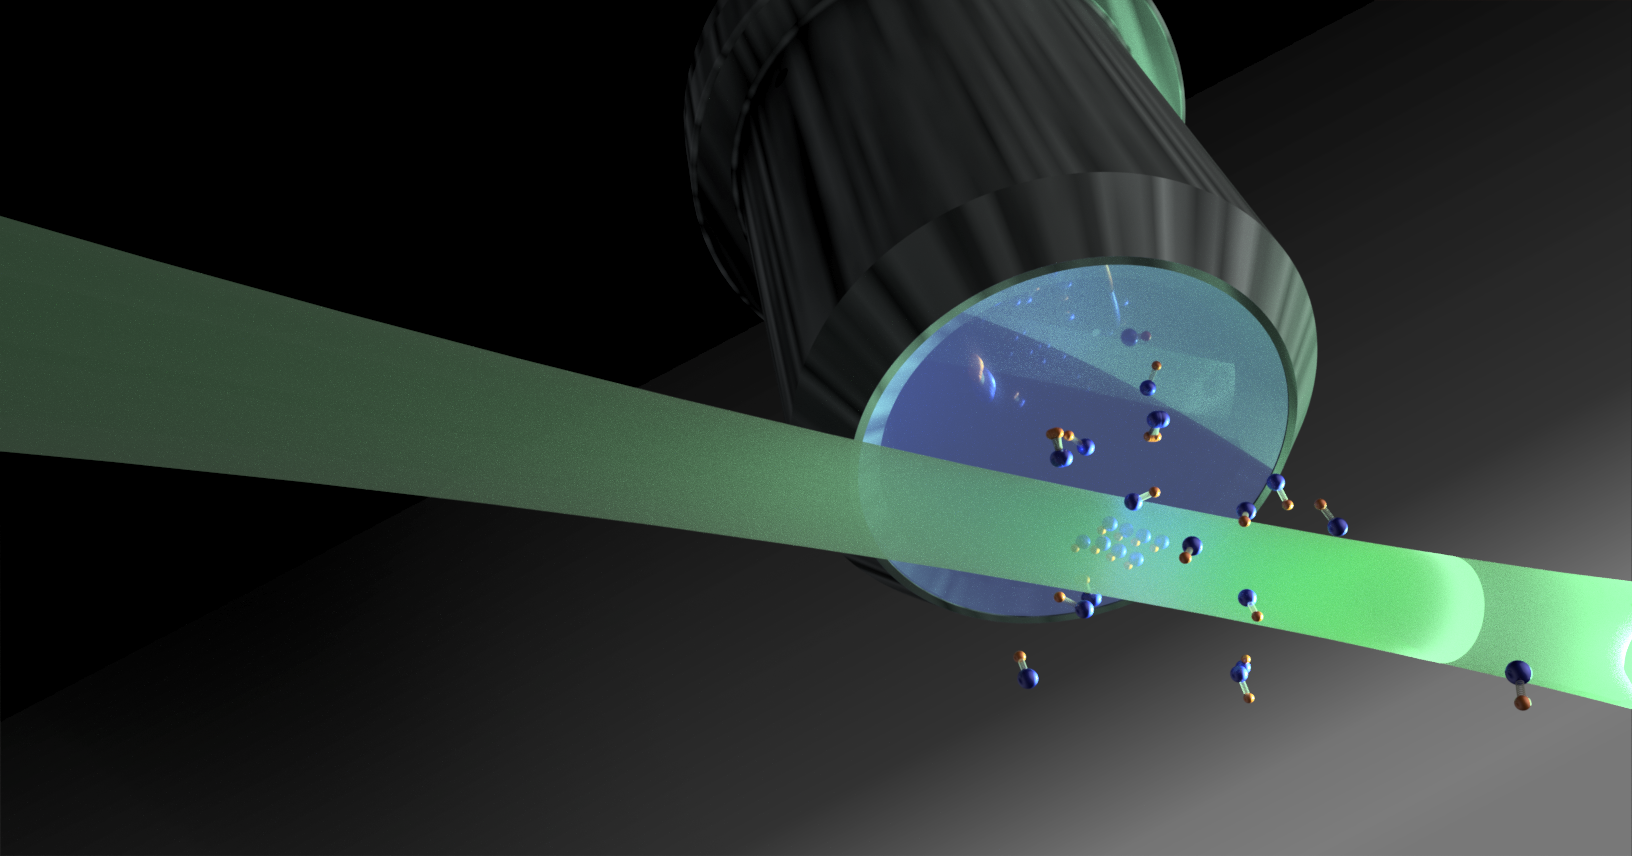
\includegraphics[width=\paperwidth]{front_bg.png}}
  }
  \setbeamercolor{title}{fg=white}
  \setbeamercolor{author}{fg=white}
  \setbeamercolor{institute}{fg=white}
  \setbeamercolor{date}{fg=white}
  \begin{frame}{}
    \titlepage
  \end{frame}
}

% % All of our experiments are done on single Na and Cs atoms in an optical tweezer.
% %% * Start with single atoms (Na and Cs) trapped from laser cooled gas
% %% * RSC and OP to prepare a single quantum state
% %% * Merge to enable interaction
% \begin{frame}[t]{}
%   \begin{center}
%     \begin{tikzpicture}[scale=0.75]
%       \mytweezer.drawCsTweezer(0, 0)
%       \mytweezer.drawNaTweezer(-1, 0)
%       \mytweezer.drawCsAtom(-0.07, 0.08, 0.22)
%       \mytweezer.drawNaAtom(-1.06, -0.09, 0.27)

%       \mytweezer.drawCsTweezer(0, -3.1)
%       \mytweezer.drawNaTweezer(-1, -3.1)
%       \mytweezer.drawCsAtom(0.0, -3.1, 0.12)
%       \mytweezer.drawNaAtom(-1.0, -3.1, 0.16)

%       \mytweezer.drawCsTweezer(-1, -7.0)
%       \mytweezer.drawNaAtom(-1.05, -6.87, 0.16)
%       \mytweezer.drawCsAtom(-0.95, -7.13, 0.12)

%       \fill[white,temporal=<1>{opacity=0.82}{opacity=0}{opacity=0.5}]
%       (-1.5, 1.5) rectangle (0.5, -1.5);
%       \fill[white,temporal=<2>{opacity=0.82}{opacity=0}{opacity=0.5}]
%       (-1.5, 1.5 - 3.1) rectangle (0.5, -1.5 - 3.1);
%       \fill[white,temporal=<3>{opacity=0.82}{opacity=0}{opacity=0.5}]
%       (-1.5, 1.5 - 7.0) rectangle (-0.5, -1.5 - 7.0);

%       \visible<2->{
%         \begin{scope}[alt=<2>{opacity=0.7}{opacity=0.35}]
%           \draw[orange,dotted,line width=1.2] (-1, -0.4) -- (-1, -2.9);
%           \draw[blue,dotted,line width=1.2] (0, -0.15) -- (0, -2.9);
%         \end{scope}
%       }

%       \visible<3->{
%         \begin{scope}[alt=<3>{opacity=0.7}{opacity=0.35}]
%           \draw[->,orange,line width=1.2] (-1, -3.3) -- (-1, -6.7);
%           \draw[->,blue,domain=-3.3:-6.7,smooth,variable=\y,line width=1.2]
%           plot ({atan((\y+4.7) * 5) / 170 - 0.5},{\y});
%         \end{scope}
%       }
%       \visible<1>{
%         \node[above,align=center] at (7, 0)
%         {\usebeamerfont{frametitle}\usebeamercolor[fg]{frametitle}{\Large Loading}};
%         \node[below,align=center] at (6.5, -0.5)
%         {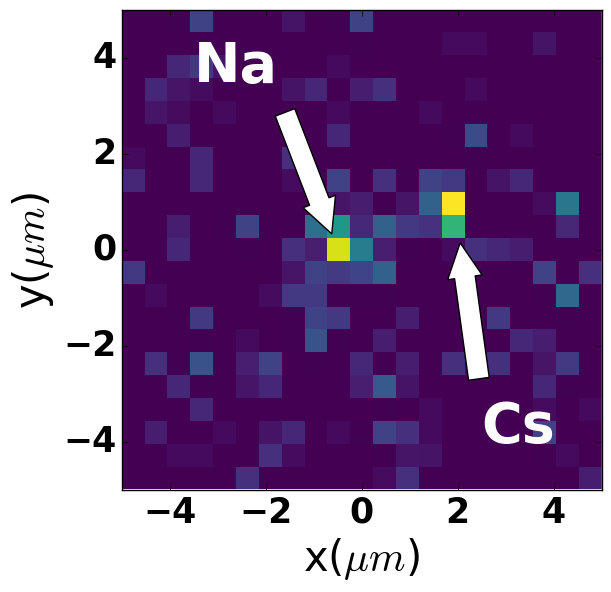
\includegraphics[width=5cm]{../../experiments/nacs_atoms/imgs/single_viridis.png}};
%         \node[below,align=center] at (7, -7.5)
%         {Loading probability per site: 60\%\\
%           Post select on initial and final state.};
%       }
%       \visible<2>{
%         \node[above,align=center] at (7, 0)
%         {\usebeamerfont{frametitle}\usebeamercolor[fg]{frametitle}{\Large Cooling}};
%         \node[below] at (6.5, -1)
%         {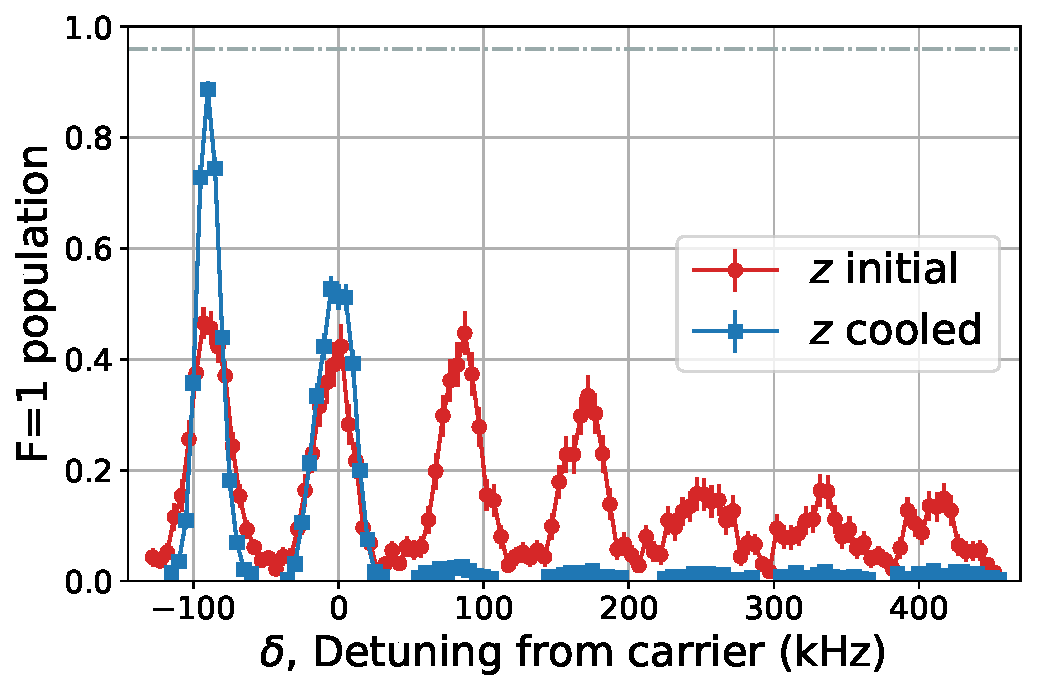
\includegraphics[width=6cm]{spectrum_nolabel_az.pdf}};
%         Don't mention axis.
%         Explain the sideband spectrum more.
%         \only<2>{
%           \node[below,align=center] at (7, -7)
%           {Cs: 96\% ground state\footnote{Phys. Rev. X 9, 021039}\\
%             Na: 94\% ground state\footnote{Phys. Rev. A 97, 063423}};
%         }
%       }
%       \visible<3>{
%         \node[above,align=center] at (7, 0)
%         {\usebeamerfont{frametitle}\usebeamercolor[fg]{frametitle}{\Large Merging}};
%         \draw[orange,line width=1.5] plot[draw,samples=200,domain=4.5:10.5]
%         function {-0.22 * exp(-(x - 9)**2 / 0.75**2) + -0.4 * exp(-(x - 6)**2 / 0.75**2) - 1};
%         \draw[blue,line width=1.5] plot[draw,samples=200,domain=4.5:10.5]
%         function {-1.2 * exp(-(x - 9)**2 / 0.75**2) + 0.45 * exp(-(x - 6)**2 / 0.75**2) - 1};
%         \mytweezer.drawNaAtom(6, -1.22, 0.15)
%         \mytweezer.drawCsAtom(9, -2.06, 0.11)

%         \draw[orange,line width=1.5] plot[draw,samples=200,domain=4.5:10]
%         function {-0.22 * exp(-(x - 7.5)**2 / 0.75**2) + -0.4 * exp(-(x - 6)**2 / 0.75**2) - 3.5};
%         \draw[blue,line width=1.5] plot[draw,samples=200,domain=4.5:10]
%         function {-1.2 * exp(-(x - 7.5)**2 / 0.75**2) + 0.45 * exp(-(x - 6)**2 / 0.75**2) - 3.5};
%         \mytweezer.drawNaAtom(6, -3.72, 0.15)
%         \mytweezer.drawCsAtom(7.5, -4.56, 0.11)

%         \draw[orange,line width=1.5] plot[draw,samples=200,domain=4.5:8.5]
%         function {-0.22 * exp(-(x - 6)**2 / 0.75**2) + -0.4 * exp(-(x - 6)**2 / 0.75**2) - 6};
%         \draw[blue,line width=1.5] plot[draw,samples=200,domain=4.5:8.5]
%         function {-1.2 * exp(-(x - 6)**2 / 0.75**2) + 0.45 * exp(-(x - 6)**2 / 0.75**2) - 6};
%         \mytweezer.drawNaAtom(5.9, -6.42, 0.12)
%         \mytweezer.drawCsAtom(6.05, -6.6, 0.13)

%         \draw[orange,line width=1.5] plot[draw,samples=200,domain=4.5:8.5]
%         function {-0.22 * exp(-(x - 6)**2 / 0.75**2) - 8.5};
%         \draw[blue,line width=1.5] plot[draw,samples=200,domain=4.5:8.5]
%         function {-1.2 * exp(-(x - 6)**2 / 0.75**2) - 8.5};
%         \mytweezer.drawNaAtom(6, -8.55, 0.14)
%         \mytweezer.drawCsAtom(6, -9.56, 0.11)

%         \draw[dotted,line width=2,black!30,opacity=10] (0.3, -3.0) -- (4.5, -0.5);
%         \draw[dotted,line width=2,black!30,opacity=10] (-0.7, -7.0) -- (4.5, -9.3);
%       }
%     \end{tikzpicture}
%     \vspace{-2cm}
%   \end{center}
% \end{frame}

% % One measurement we can do is the scattering length
% %% between Na and Cs since it captures many aspects of the atom-atom interaction
% %% * Binding energy
% %% * Molecular potential
% %% * Feshbach resonance
% %% * Molecule formation
% \begin{frame}{Scattering length $a$}
%   \begin{columns}
%     \column{4.5cm}
%     \begin{itemize}
%     \item<2-> Binding energy
%     \item<3-> Molecular potential
%     \item<4-> Feshbach resonance
%     \item<5-> Molecule formation\\
%       $\vdots$
%     \end{itemize}
%     \column{6.5cm}
%     \begin{tikzpicture}
%       \begin{scope}[scale=0.65]
%         \draw[->,line width=1.2] (0, 0) -- (0, 8);
%         \node[above,rotate=90] at (0, 4) {Energy};
%         \draw[->,line width=1.2] (0, 0) -- (8, 0);
%         \node[below] at (4, -0.5) {Internuclear distance};

%         \draw[dashed] (1.0269 - 0.25, 2.5) -- (7 - 0.25, 2.5);
%         \draw (1.0793 - 0.25, -0.4631 + 2.5) -- (4.5 - 0.25, -0.4631 + 2.5);

%         \draw[line width=1.1]
%         plot[samples=200,domain=0.8:7,variable=\x]
%         ({\x - 0.25}, {6.8*\x^(-3.4)-6.5*\x^(-1.7) + 2.5});

%         \mytweezer.drawNaAtom(5.55, 2.7, 0.12)
%         \mytweezer.drawCsAtom(6.05, 2.7, 0.10)

%         \mytweezer.drawNaAtom(2.08, 2.15, 0.12)
%         \mytweezer.drawCsAtom(2.25, 2.15, 0.10)

%         \draw[->, cyan!50!blue, line width=0.8] (5.4, 2.7) -- ++(-3.5, 0)
%         arc (270:90:0.2) -- ++(2.5, 0);
%       \end{scope}
%     \end{tikzpicture}
%   \end{columns}
% \end{frame}

%% We measure the scattering length using interaction shift.
%% When we successfully loaded two atoms in the tweezer,
%% their energy levels will be shifted due to the interaction.
%% This shift depends on the spin state of the atom and we can measure this difference
%% by driving a Raman or microwave transition between HF states.
%% As shown.... by comparing the spectrum with and without another atom...
%% This way of measuring the scattering length is similar to the experiement done
%% in optical lattice on Mott insulator but the anisotropy causes some difference as shown in.

% Interaction shift data
%% One peak on the right, lowering energy -> attractive interaction.
%% Another peak on the left...
%% Significant state mixing due to low axial trapping frequency
%% Theory model
%% 33+22 -> 33+11

% \begin{frame}{Interaction shift}
%   \vspace{-0.8cm}
%   \begin{tikzpicture}
%     \draw[white,opacity=0] (-6, -4.5) rectangle (6, 4.5);
%     % Raman sequence
%     \visible<1>{
%       \node at (-2.8, 0.7) {\includegraphics[width=6cm]{shift_raman_1.pdf}};
%     }
%     \visible<2-3>{
%       \node at (-2.8, 0.7) {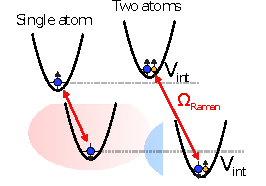
\includegraphics[width=6cm]{shift_raman.pdf}};
%     }
%     % Data 1
%     \visible<3-6>{\node at (3.2, 0) {\includegraphics[width=5cm]{na2cs4_0.pdf}};}
%     \visible<7>{\node at (3.2, 0) {\includegraphics[width=5cm]{na2cs4.pdf}};}
%     \visible<8->{\node at (3.2, 0) {\includegraphics[width=5cm]{na2cs3.pdf}};}

%     % Equations
%     \visible<4-5>{
%       \node[below right,align=left] at (-4.9, 3.8)
%       {\footnotesize $\displaystyle H=\!\!\sum_{i=x,y,z}(\frac{m_{1}\omega_{1,i}^2x_{1,i}^2}{2}+\frac{p_{1,i}^2}{2m_{1}})\ +\!\sum_{i=x,y,z}(\frac{m_{2}\omega_{2,i}^2x_{2,i}^2}{2}+\frac{p_{2,i}^2}{2m_{2}})+V_{int}(\vec r_1-\vec r_2)$};
%       \draw[decoration={brace,mirror,amplitude=10pt},decorate,line width=1]
%       (-4.15,2.8) -- node[below=10pt] {\small Na} (-1.15,2.8);
%       \draw[decoration={brace,mirror,amplitude=10pt},decorate,line width=1]
%       (-0.5,2.8) -- node[below=10pt] {\small Cs} (2.5,2.8);
%       \draw[decoration={brace,mirror,amplitude=10pt},decorate,line width=1]
%       (3.05,3) -- node[below=10pt] {\small Interaction} (4.55,3);
%     }
%     \visible<5>{
%       \node[above right,align=left] at (-5.8, -2.3)
%       {
%         \textcolor{blue!60!black}{To center of mass}\\
%         \textcolor{blue!60!black}{and relative coordinates}\\
%         \\
%         {\tiny
%           $\begin{aligned}
%             M=&\ m_1+m_2&\mu=&\ \frac{m_1m_2}{m_1+m_2}\\
%             \Omega_i^2=&\ \frac{m_1\omega_{1,i}^2+m_2\omega_{2,i}^2}{m_1+m_2}&\omega_{R,i}^2=&\ \frac{m_2\omega_{1,i}^2+m_1\omega_{2,i}^2}{m_1+m_2}\\
%             X_i=&\ \frac{m_1x_{1,i}+m_2x_{2,i}}{m_1+m_2}&x_{R,i}=&\ x_{1,i}-x_{2,i}\\
%             P_i=&\ p_{1,i}+p_{2,i}&p_{R,i}=&\ \frac{m_2p_{1,i}-m_1p_{2,i}}{m_1+m_2}
%           \end{aligned}$}};
%     }
%     \visible<5->{
%       \node[above right,align=left] at (-6, -4.5)
%       {\footnotesize $\displaystyle H=\!\!\sum_{i=x,y,z}(\frac{M\Omega_{i}^2X_{i}^2}{2}+\frac{P_{i}^2}{2M})\ +\!\sum_{i=x,y,z}(\frac{\mu\omega_{R,i}^2x_{R,i}^2}{2}+\frac{p_{R,i}^2}{2\mu})+V_{int}(\vec r_R)\ +\!\sum_{i=x,y,z}\mu(\omega_{1,i}^2 - \omega_{2,i}^2)X_ix_{R,i}$};
%       \draw[decoration={brace,amplitude=10pt},decorate,line width=1]
%       (-5.25,-3.5) -- node[above=10pt] {\small Center of mass} (-2.5,-3.5);
%       \draw[decoration={brace,amplitude=10pt},decorate,line width=1]
%       (-1.9,-3.5) -- node[above=10pt] {\small Relative} (2.4,-3.5);
%       \draw[decoration={brace,amplitude=10pt},decorate,line width=1]
%       (3,-3.5) -- node[above=10pt] {\small Mixing} (5.9,-3.5);
%     }
%     \visible<6>{
%       \node at (-2.6, 0.5) {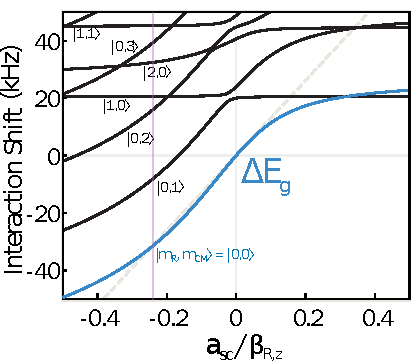
\includegraphics[width=6cm]{shift_theory.pdf}};
%     }
%     \visible<7>{
%       \node at (-2.6, 0.5) {\includegraphics[width=6cm]{shift_theory42_32.pdf}};
%     }
%     \visible<8->{
%       \node at (-2.6, 0.5) {\includegraphics[width=6cm]{shift_theory32_31.pdf}};
%     }
%     \visible<9->{
%       \fill[white,opacity=0.95] (-6, -4.5) rectangle (6, 3.5);
%       \node[align=center] at (0, 2.1)
%       {Combined with binding energy measurement on Na(2,2) Cs(4,4)\\
%         \\
%         \begin{tabular}{|c|c|}
%           \hline
%           Spin state ($F,m_F$)&Scattering length (a.u.)\\\hline
%           Na(2,2) Cs(4,4)&30.36\\\hline
%           Na(2,2) Cs(3,3)&-693.8\\\hline
%           Na(1,1) Cs(3,3)&13.19\\\hline
%         \end{tabular}};
%     }
%     \visible<10->{
%       \draw[->, line width=1, color=red!50!black] (0.8, 1.45) -- (-2, 0.5)
%       node[below] {Enhanced coupling to molecular state?};
%     }
%     \visible<11->{
%       \node at (1.3, -2) {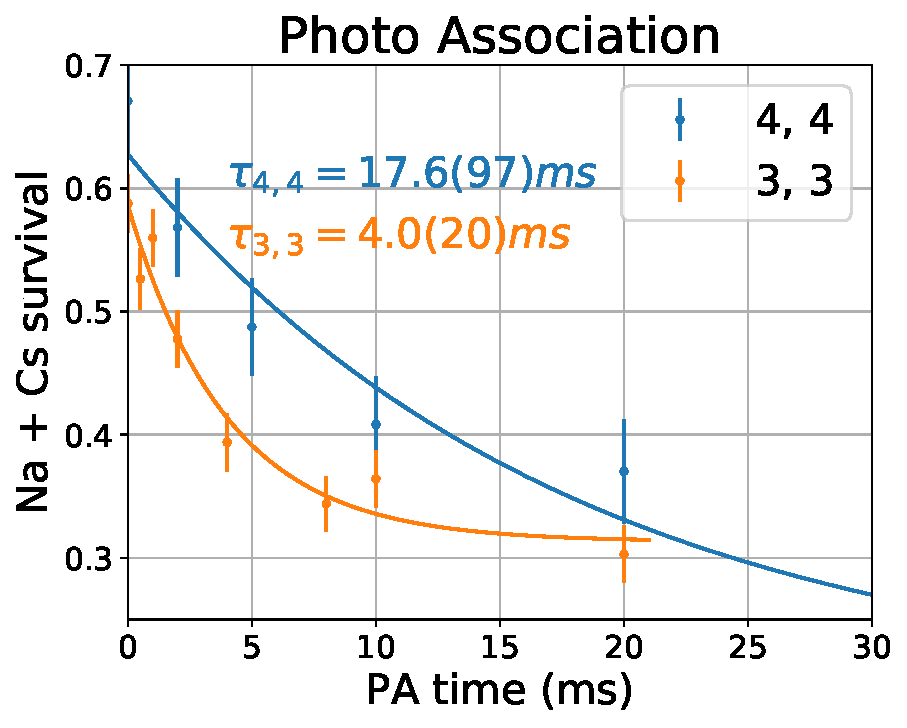
\includegraphics[width=5cm]{../../experiments/nacs_201904/imgs/data_20190521_lifetime_cmp_lin.pdf}};
%     }
%   \end{tikzpicture}
% \end{frame}

% Another thing we can measure is the FB resonance
%% Better prediction than before.
% \begin{frame}[t]{Na (1, -1) Cs (3, -3) Feshbach resonance}
%   \only<1>{
%     \begin{center}
%       \includegraphics[height=7cm]{chamber1_5.jpg}
%     \end{center}
%   }
%   \only<2->{
%     \begin{center}
%       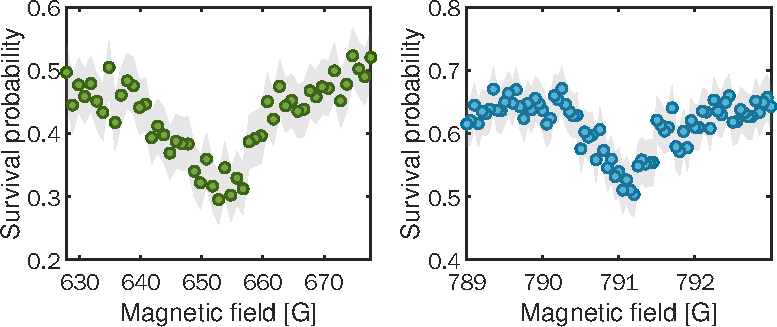
\includegraphics[width=10cm]{fb.pdf}\\
%       \vspace{0.5cm}
%     \end{center}
%   }
%   \only<3->{
%     \begin{center}
%       \begin{tabular}{|c|p{1.9cm}|p{1.9cm}|}
%         \hline
%         &$s$-wave&$p$-wave\\\hline
%         Predicted {\tiny (based on interaction shift)\footnote{In collaboration with Bo Gao}}&$663$ G&$799$ G\\\hline
%         Measured&$652(3)$ G&$791.2(2)$ G\\\hline
%       \end{tabular}
%     \end{center}
%   }
% \end{frame}

% \begin{frame}{Conclusion}
%   \begin{center}
%     \begin{itemize}
%     \item Interaction shift of Na and Cs
%     \item Feshbach resonance Na(1,-1) Cs(3,-3)
%     \end{itemize}
%     \vspace{1cm}
%     \visible<2->{
%       {\usebeamerfont{frametitle}\usebeamercolor[fg]{frametitle}{Next step}}
%       \begin{itemize}
%       \item Make Feshbach molecules
%       \item Optical molecule formation taking advantage of the large scattering length
%       \end{itemize}
%       \vspace{1cm}
%     }
%     \visible<3->{
%       Thank you for your attention.\\
%       % Poster
%       Poster S01.00155 (Thursday afternoon)
%     }
%   \end{center}
% \end{frame}

\end{document}
